\documentclass[11pt]{article}

% --------------------
% PACOTES ESSENCIAIS
% --------------------
\usepackage[utf8]{inputenc}     % Codificação UTF-8
\usepackage[T1]{fontenc}        % Fonte com acentuação
\usepackage[brazil]{babel}      % Idioma português
\usepackage{amsmath, amssymb}   % Símbolos matemáticos
\usepackage{graphicx}           % Inserção de imagens
\usepackage{geometry}           % Margens personalizadas
\usepackage{fancyhdr}           % Cabeçalhos e rodapés
\usepackage{enumitem}           % Listas personalizadas
%\usepackage{physics}            % Notação física e matemática
\usepackage{hyperref}           % Links no PDF
\usepackage{multicol}           % Colunas (opcional)
\usepackage{xcolor}
\usepackage{siunitx}
\usepackage{comment}

\newtheorem{destaque}{Destaque}

% --------------------
% CONFIGURAÇÕES
% --------------------
\geometry{a4paper, margin=2.5cm}

\pagestyle{fancy}
\fancyhf{}
\rhead{Integrais de linha}
\lhead{Caio Magno Mendonça Nicácio}
\cfoot{\thepage}

\setlength{\parskip}{0.5em}
\setlength{\parindent}{0pt}

% --------------------
% INÍCIO DO DOCUMENTO
% --------------------
\begin{document}
	
	\begin{center}
		\Large\textbf{INTEGRAIS DE LINHA} \\
		\normalsize
		Data: \today
	\end{center}
	
	\hrule
	\vspace{1em}
	
	\tableofcontents
	\newpage
	
	\section{Curvas e parametrização}
	
	Seja $\gamma:[a, b]\to \Omega$. Uma parametrização de $\gamma$ é uma função, tal que,
	\begin{gather*}
		\boldsymbol{\vec{r}}:\Omega \subseteq \mathbb{R}\to \mathbb{R}^n \\
		\boldsymbol{\vec{r}}(t)=(x_1(t),\, x_2(t),\, \cdots,\, x_n(t)),
	\end{gather*}
	cuja imagem de $\boldsymbol{\vec{r}}$ é exatamente a curva $\gamma$ (Fig. \ref{fig:parametrizacao}). Verifica-se, portanto, que
	\begin{equation*}
		\gamma=\{\boldsymbol{\vec{r}}(t)\in \mathbb{R}^n: t\in [a,b]\}.
	\end{equation*}
	Uma mesma curva $\gamma$ pode ter infinitas parametrizações, as quais descrevem a mesma curva $\gamma$, mas cuja configuração influencia na velocidade e sentido em que é percorrida.
	\begin{figure}[h!]
		\centering
		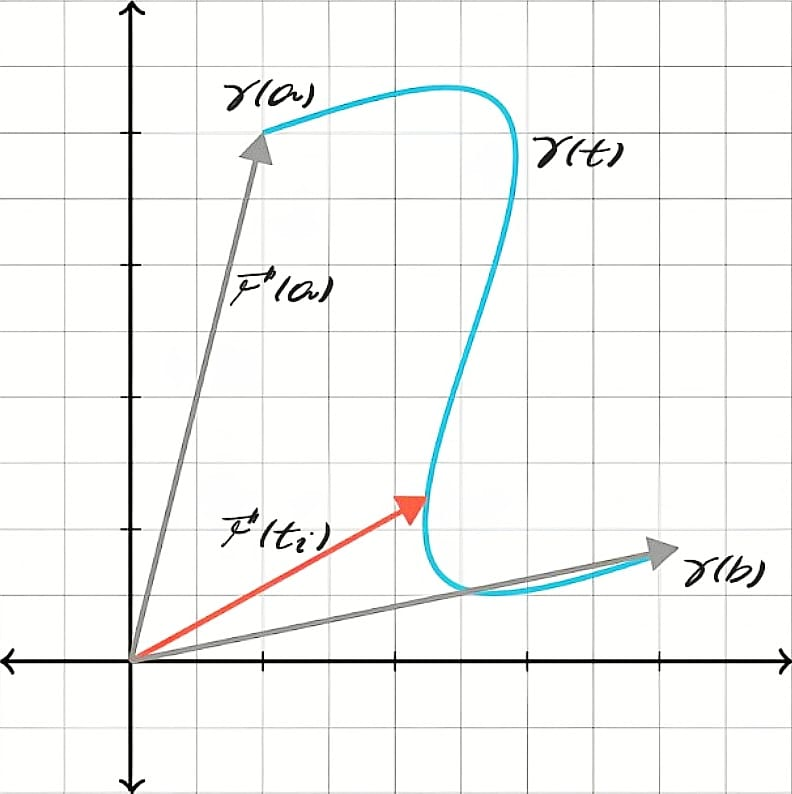
\includegraphics[width=5.5cm]{figure/parametrizacao.jpeg}
		%\captionsetup{width=16cm}
		\caption{\centering Parametrização arbitrária $\boldsymbol{\vec{r}}(t)$ cuja imagem é a curva $\gamma(t):[a, b]$.}
		\label{fig:parametrizacao}
	\end{figure}

	As parametrizações
	\begin{align*}
		\boldsymbol{\vec{r}}_1&=(\cos t, \sin t, t)\\
		\boldsymbol{\vec{r}}_2&=(\cos 2t, \sin 2t, t) \\
		\boldsymbol{\vec{r}}_3&=(\cos t, \sin t, t/2) \\
		\boldsymbol{\vec{r}}_4&=(\cos 2t, \sin 2t, t/2),
	\end{align*}
	associadas às Fig. \ref{fig:curvas-circulo}a, \ref{fig:curvas-circulo}b, \ref{fig:curvas-circulo}c e \ref{fig:curvas-circulo}d, respectivamente, descrevem a mesma projeção da curva $\gamma=\{(x,y):x^2+y^2=1\}$, $\gamma:[a,b]\to \Omega$ no plano $\mathbb{R}^2$, que passam pelos mesmos pontos $(x,y)$. 
	
	\begin{figure}[h!]
		\begin{minipage}[b]{0.24\textwidth}
			\centering
			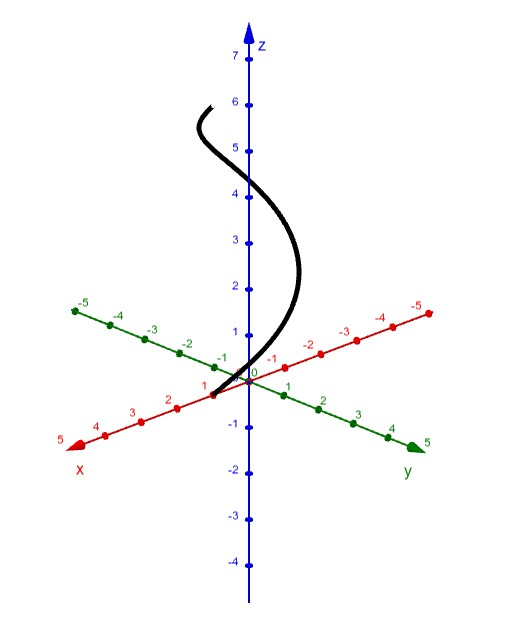
\includegraphics[width=\textwidth]{figure/curva-1.jpeg}
			\\[-1ex]\small (a)
		\end{minipage}
		\hfill
		\begin{minipage}[b]{0.24\textwidth}
			\centering
			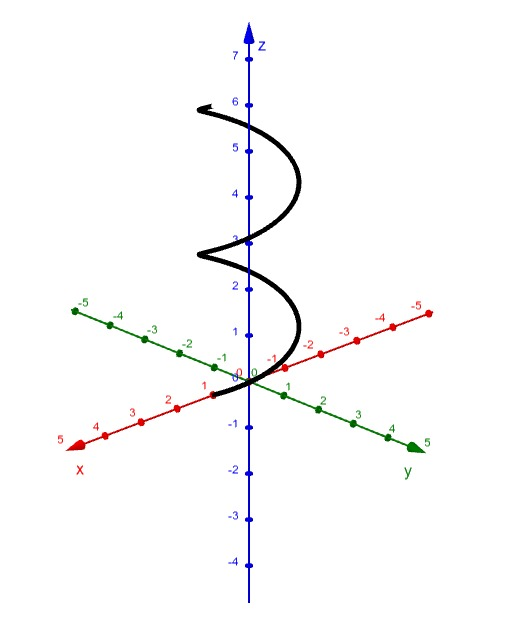
\includegraphics[width=\textwidth]{figure/curva-2.jpeg}
			\\[-1ex]\small (b)
		\end{minipage}
		\hfill
		\begin{minipage}[b]{0.24\textwidth}
			\centering
			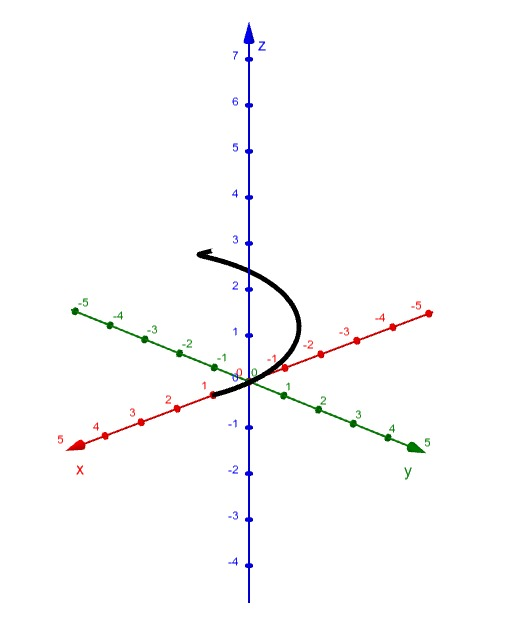
\includegraphics[width=\textwidth]{figure/curva-3.jpeg}
			\\[-1ex]\small (c)
		\end{minipage}
		\hfill
		\begin{minipage}[b]{0.24\textwidth}
			\centering
			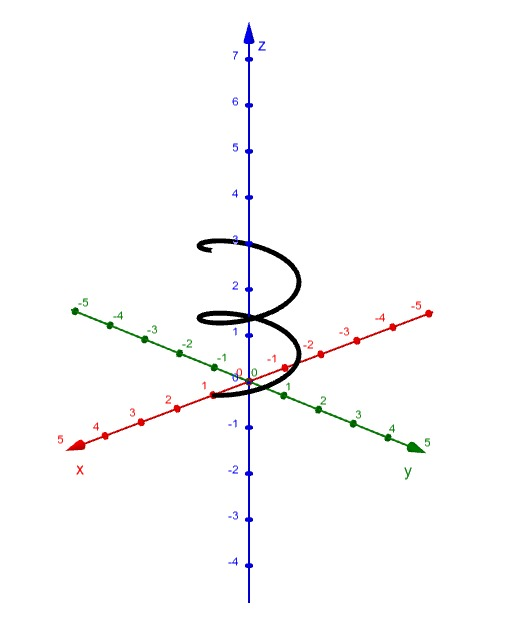
\includegraphics[width=\textwidth]{figure/curva-4.jpeg}
			\\[-1ex]\small (d)
		\end{minipage}
		\centering
		%\captionsetup{width=16cm}
		\caption{\centering Parametrizações $\boldsymbol{\vec{r}}_i$, $i=1,2,\cdots,n$, com mesma projeção no plano $xy$.}
		\label{fig:curvas-circulo}
	\end{figure}
	
	A Figura \ref{fig:gamma-r2} é projeção de $\gamma$ no $\mathbb{R}^2$, descrita por várias parametrizações. O eixo $z$ na Fig. \ref{fig:curvas-circulo} é o tempo, enquanto $\lambda(t)$ em $\boldsymbol{\vec{r}}(\lambda(t))=(\cos \lambda(t), \sin \lambda(t))$ governa a velocidade em função do tempo\footnote{A quantidade de vezes no qual a curva foi percorrida em um mesmo intervalo $\Delta t$.}.
	
	\begin{destaque}
		$\gamma$ é um conjunto de pontos no espaço $\mathbb{R}^n$, em que a parametrização é uma maneira específica de descrever uma ordem para visitar esses pontos.
	\end{destaque}
	
	\begin{figure}[h!]
		\centering
		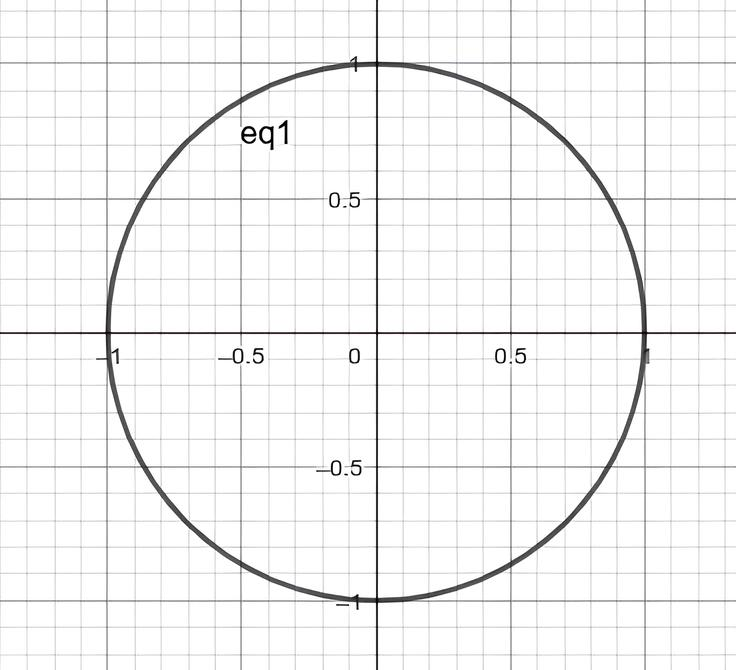
\includegraphics[width=6.5cm]{figure/gamma-r2.jpeg}
		%\captionsetup{width=16cm}
		\caption{\centering Projeção da curva $\gamma$ segundo diversas parametrizações $\boldsymbol{\vec{r}}$ presentes na Fig. \ref{fig:curvas-circulo}.}
		\label{fig:gamma-r2}
	\end{figure}

	Seja $\boldsymbol{\vec{r}}(\lambda(t))=(\cos \lambda(t), \sin \lambda(t))$ uma parametrização da curva $\gamma$. $\lambda(t)$ governa como a projeção circular é percorrida ao longo do eixo $z=t$. Logo, é conveniente interpretar $t$ como o tempo e $\lambda(t)$ como o coeficiente angular no plano $xy$, em função do tempo. A velocidade angular da projeção é, portanto,
	\begin{gather*}
		\omega(t)=\frac{d\lambda}{dt}(t)=\lambda'(t), \quad [\omega(t)]=\frac{\text{rad}}{\text{s}}.
	\end{gather*}

	A frequência vertical, a cada volta completa, é
	\begin{gather*}
		f=\frac{2\pi}{\lambda'(t)},\quad \lambda'(t)\in \mathbb{R}, \quad [f]=\text{s}^{-1}.
	\end{gather*}

	\section{Integral de linha de primeira espécie}
	\label{sec:integral-linha-1}
	
	Seja $f:\Omega \subset \mathbb{R}^m\to \mathbb{R}^n$ uma função escalar aplicada ao longo de uma curva $\gamma:[a,b]\to \mathbb{R}^2$.
	A expressão
	\begin{equation*}
		\int_{\gamma} f(x,y)\, ds
	\end{equation*}
	denota uma integral de linha de $f$ sobre $\gamma(t)$, onde $x=x(t)$ e $y=y(t)$. Imediatamente, tem-se que
	\begin{equation}
		\int_{\gamma} f(x(t),y(t))\, ds=\int_{\gamma} f(x(t),y(t))\, \sqrt{\left(\frac{dx}{dt}\right)^2+\left(\frac{dy}{dt}\right)^2}\, dt,
		\label{eq:integral-primeira-especie}
	\end{equation}
	em que $ds$ é o comprimento infinitesimal de arco $\Delta s_i\to 0$ (Fig. \ref{fig:integral-primeira-especie}).
	\begin{figure}[h!]
		\centering
		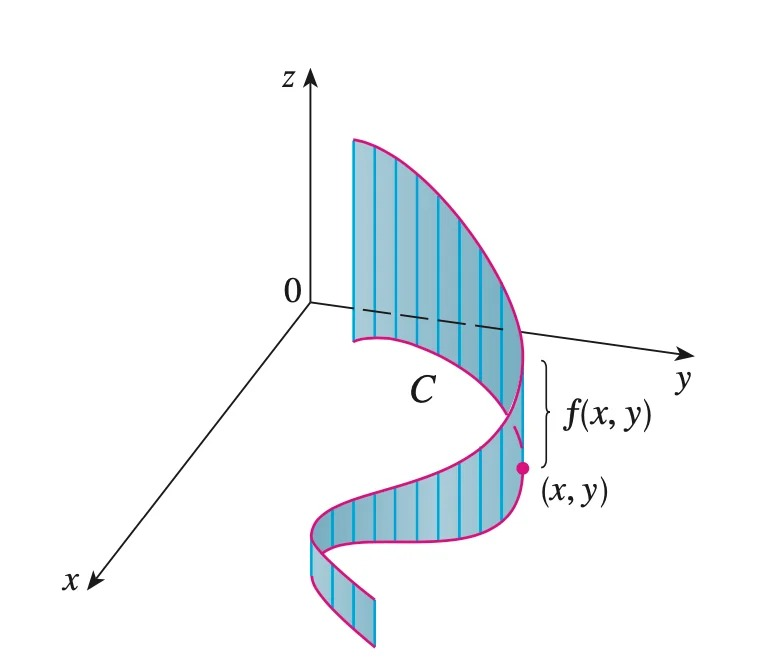
\includegraphics[width=7cm]{figure/integral-primeira-especie.jpeg}
		%\captionsetup{width=16cm}
		\caption{\centering Integral de linha de uma função $f:\Omega \subset \mathbb{R}^2$ aplicada a uma curva $C\to \Omega$.}
		\label{fig:integral-primeira-especie}
	\end{figure}
	
	Nota-se que, para definir a integral, não é necessário que $f$ esteja definida fora da imagem de $\gamma$.
	
	\section{Integral de linha de segunda espécie}
	\label{sec:integral-linha-2}
	
	Seja $\boldsymbol{\vec{F}}:\Omega \subset \mathbb{R}^2\to \mathbb{R}^2$ um campo de forças definido no aberto $\Omega$ e que uma partícula descreva um movimento em $\Omega$ com função de posição $\gamma:[a, b]\to \Omega$. $\gamma(t)$ representa a posição da partícula 
	no instante $t$.
	
	Se $\boldsymbol{\vec{F}}$ for constante e a imagem de $\gamma$ um segmento, o trabalho, $\tau$, realizado por $\boldsymbol{\vec{F}}$ de $\gamma(a)$ até $\gamma(b)$ é, por definição, o produto escalar de $\boldsymbol{\vec{F}}$ pelo deslocamento $\gamma(b)-\gamma(a)$.
	\begin{gather*}
		\tau=\boldsymbol{\vec{F}}\cdot [\gamma(b)-\gamma(a)] \\
		\tau=|\boldsymbol{\vec{F}}|\, |\gamma(b)-\gamma(a)|\, \cos \theta
	\end{gather*}
	Sejam $\boldsymbol{\vec{F}}$ contínuo e $\gamma \in C^1$. Deseja-se definir o trabalho $\tau$ realizado por $\boldsymbol{\vec{F}}$ de $\gamma(a)$ até $\gamma(b)$. Seja $P:[a,b]$ uma partição contínua do domínio, no qual o intervalo entre cada item é infinitesimal, $\Delta t_i$ suficientemente pequeno (Fig. \ref{fig:trabalho}).
	
	\begin{figure}[h!]
		\centering
		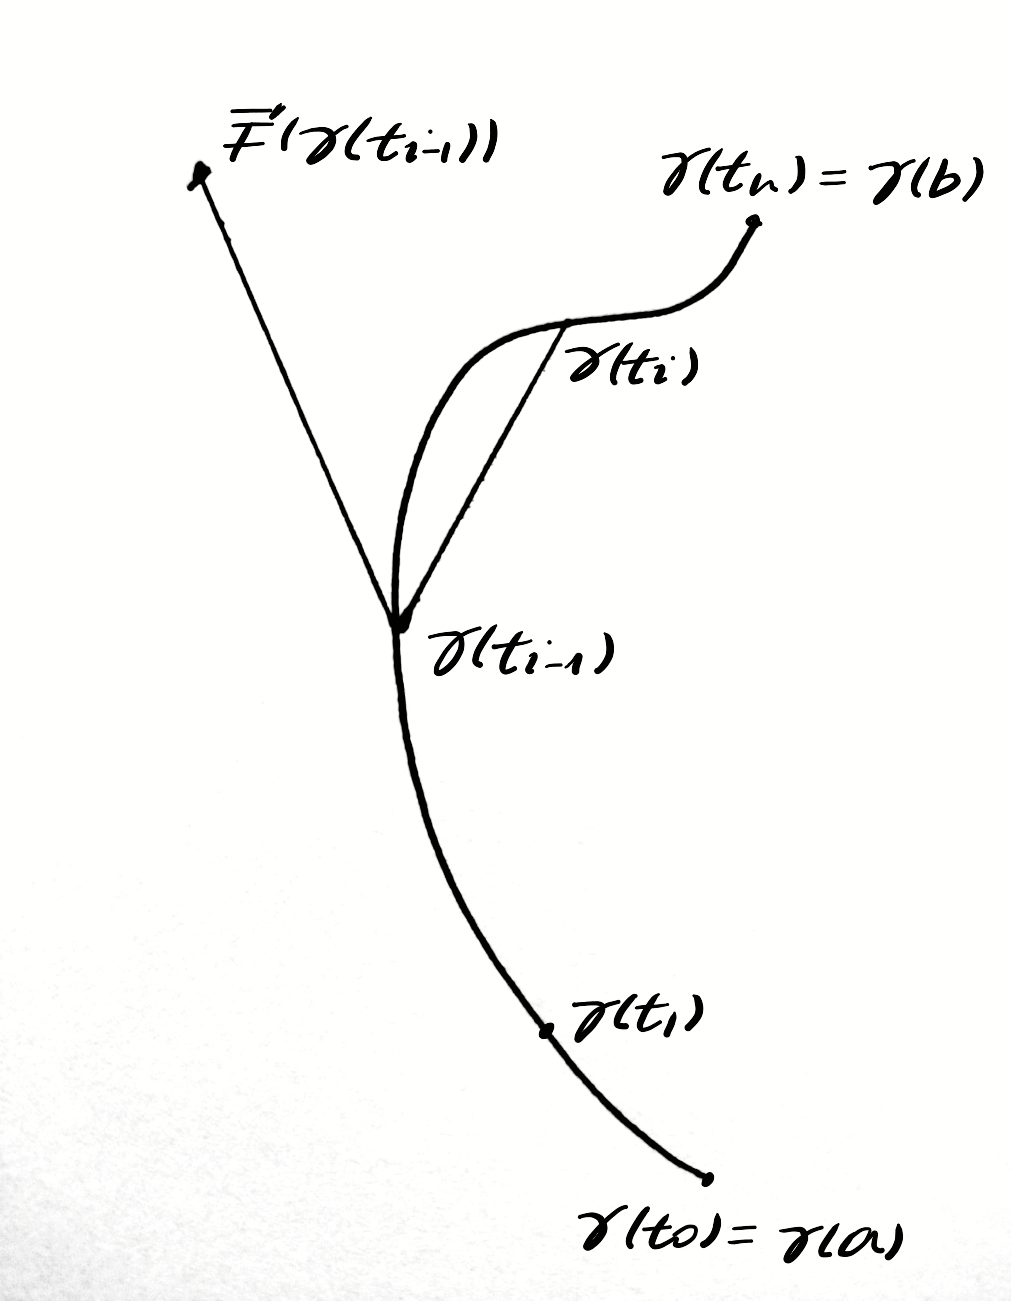
\includegraphics[width=5.5cm]{figure/trabalho.jpg}
		%\captionsetup{width=16cm}
		\caption{\centering Força $\boldsymbol{\vec{F}}(\gamma(t_{i-1}))$ aplicada a uma distância infinitesimal $\gamma(t_i)-\gamma(t_{i-1})$.}
		\label{fig:trabalho}
	\end{figure}
	
	É razoável considerar que
	\begin{equation}
		\tau=\sum_{i=1}^{n} \boldsymbol{\vec{F}}(\gamma (t_{i-1}))\cdot [\gamma(t_i)-\gamma(t_{i-1})]
		\label{eq:tau-1}
	\end{equation}
	seja uma boa aproximação para o trabalho $\tau$ realizado por $\boldsymbol{\vec{F}}$ de $\gamma(a)$ até $\gamma(b)$ e que esta aproximação seja tanto melhor quando menor for o intervalo máx $\Delta t_i$. Assim,
	\begin{gather}
		\frac{d\gamma}{dt}(t_{i-1})=\lim_{\Delta t_i\to 0} \frac{\gamma(t_i)-\gamma(t_{i-1})}{\Delta t_i} \nonumber\\
		\frac{d\gamma}{dt}(t_{i-1})\approx \frac{\gamma(t_i)-\gamma(t_{i-1})}{\Delta t_i} \nonumber\\
		\gamma(t_i)-\gamma(t_{i-1})\approx \frac{d\gamma}{dt}(t_{i-1})\, \Delta t_i.
		\label{eq:tau-2}
	\end{gather}
	Logo, substituindo a Eq. \ref{eq:tau-2} na Eq. \ref{eq:tau-1}, é obtido
	\begin{equation*}
		\tau\approx \sum_{i=1}^{n}\boldsymbol{\vec{F}}(\gamma(t_{i-1}))\cdot \frac{d\gamma}{dt}(t_{i-1})\, \Delta t_i.
	\end{equation*}
	Como $\boldsymbol{\vec{F}}\cdot \frac{d\gamma}{dt}$ em $[a,b]$ é integrável e contínua no intervalo, segue que
	\begin{equation*}
		\lim_{\text{máx}\, \Delta t_i\to 0} \tau=\lim_{\text{máx}\, \Delta t_i\to 0} \sum_{i=1}^{n} \boldsymbol{\vec{F}}(\gamma (t_{i-1}))\cdot [\gamma(t_i)-\gamma(t_{i-1})]=\int_{a}^{b} \boldsymbol{\vec{F}}(\gamma(t))\cdot\frac{d\gamma}{dt}(t)\, dt.
	\end{equation*}
	Portanto, o trabalho realizado por $\boldsymbol{\vec{F}}$ de $\gamma(a)$ até $\gamma(b)$ pode ser definido por
	\begin{equation*}
		\tau=\int_{a}^{b} \boldsymbol{\vec{F}}(\gamma(t))\cdot\frac{d\gamma}{dt}(t)\, dt,
	\end{equation*}
	em que $\int_{a}^{b} \boldsymbol{\vec{F}}\cdot d\gamma$ é a notação para indicar a integral $\int_{a}^{b} \boldsymbol{\vec{F}}(\gamma(t))\cdot\frac{d\gamma}{dt}(t)\, dt$.
	
	Sejam $\boldsymbol{\vec{F}}:\Omega \subset \mathbb{R}^n\to \mathbb{R}^n$ e $\gamma\in C^1$. A integral de linha de $\boldsymbol{\vec{F}}$ sobre $\gamma$ é definida por
	\begin{equation}
		\int_{a}^{b} \boldsymbol{\vec{F}}\cdot d\gamma=\int_{a}^{b} \left\langle \boldsymbol{\vec{F}}(\gamma(t)), \frac{d\gamma(t)}{dt}\, dt \right\rangle.
		\label{eq:integral-linha}
	\end{equation}
	
	\begin{comment}
		\begin{figure}[h!]
			\begin{minipage}[b]{0.48\textwidth}
				\centering
				
\includegraphics[width=\textwidth]{figure/estado-geral-tensao-1.png}
				\\[-1ex]\small (a)
				\label{fig:estado-geral-1}
			\end{minipage}
			\hfill
			\begin{minipage}[b]{0.48\textwidth}
				\centering
				
\includegraphics[width=\textwidth]{figure/estado-geral-tensao-2.png}
				\\[-1ex]\small (b)
				\label{fig:estado-geral-2}
			\end{minipage}
			\centering
			%\captionsetup{width=16cm}
			\caption{\centering Representação do estado geral de tensões em um ponto $Q$: (a) no sistema de coordenadas original e (b) no sistema resultante de uma rotação em relação ao sistema inicial.}
			\label{fig:estado-geral}
		\end{figure}
	\end{comment}
	
	%\bibliography{pos-textuais/referencias.bib}
	
\end{document}